% generated by scripts/pkl_to_latex.py
% source PKL : uscan_v1_L4_Ne4_t1_mode-uniform_nmin2_solver-gcg_full_restarts2_iter40_kmax1_tol1em09_U0to4_N3-4ce234abfbe0.pkl
% scan type  : uscan
% state      : gs
% requires   : \usepackage{pgfplots} \pgfplotsset{compat=1.18}
% colours match the matplotlib PDF (tab10 cycle)
\definecolor{gmeC0}{HTML}{1F77B4}
\definecolor{gmeC1}{HTML}{FF7F0E}
\definecolor{gmeC2}{HTML}{2CA02C}
\definecolor{gmeC3}{HTML}{D62728}
\definecolor{gmeC4}{HTML}{9467BD}
\definecolor{gmeC5}{HTML}{8C564B}
\definecolor{gmeC6}{HTML}{E377C2}
\definecolor{gmeC7}{HTML}{17BECF}

\begin{figure}[htbp]
  \centering
  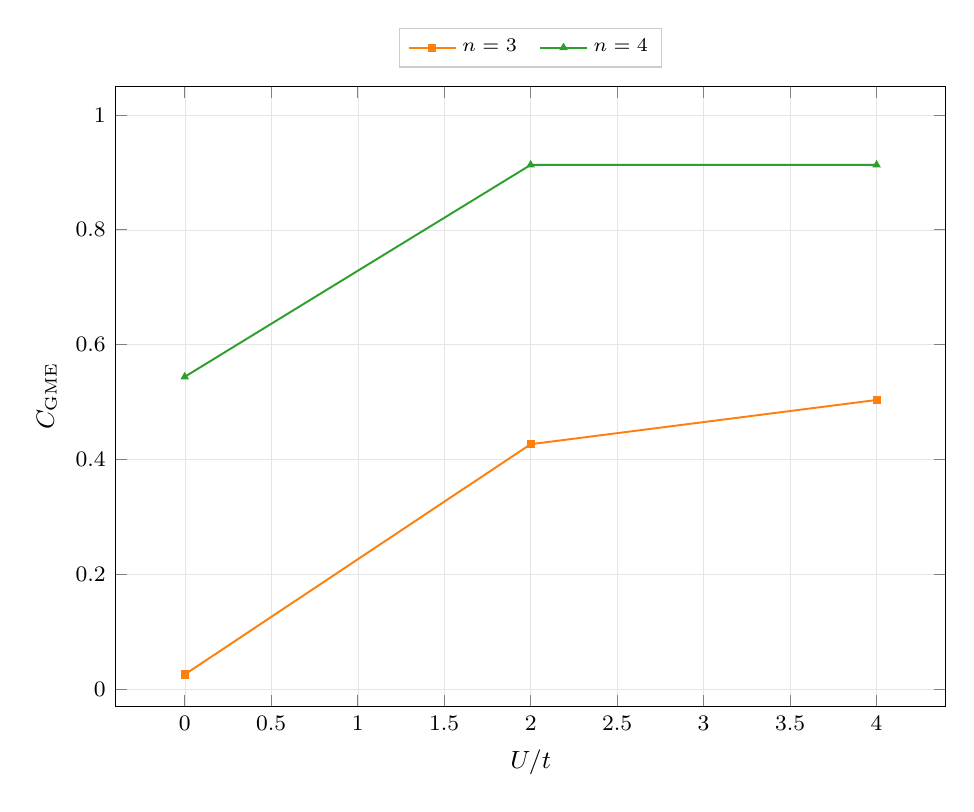
\begin{tikzpicture}
    \begin{axis}[
      width=\columnwidth,
      height=0.78\columnwidth,
      xlabel={$U/t$},
      ylabel={$C_{\mathrm{GME}}$},
      grid=both,
      grid style={line width=.1pt, draw=gray!20},
      tick label style={font=\footnotesize\rmfamily, /pgf/number format/fixed},
      label style={font=\small\rmfamily},
      scaled ticks=false,
      legend style={font=\scriptsize\rmfamily, draw=gray!40, at={(0.5,1.03)}, anchor=south, /tikz/every even column/.append style={column sep=6pt}},
      legend cell align={left},
      legend columns=2,
      ymin=-0.03,
      ymax=1.05,
    ]
      \addplot[color=gmeC1, mark=square*, mark size=1.1pt, line width=0.7pt] coordinates {
          (0,0.025431) (2,0.426456) (4,0.503514)
      };
      \addlegendentry{$n=3$}
      \addplot[color=gmeC2, mark=triangle*, mark size=1.1pt, line width=0.7pt] coordinates {
          (0,0.543826) (2,0.912871) (4,0.912871)
      };
      \addlegendentry{$n=4$}
    \end{axis}
  \end{tikzpicture}
  \caption{Spin entanglement in the ground state of the Hubbard ring as a function of $U/t$, for different values of the spin number $n$, with $K=L$ and $V=0$.}
  \label{fig:uscan-gs-l4-k4-b8b1d9}
\end{figure}
